% small.tex
\documentclass{beamer}
%\usetheme{default}
\usetheme{Warsaw}
\usecolortheme{whale}
\usepackage{tikz}
\usepackage[absolute,overlay]{textpos}
\usepackage{soul}
\usepackage{pdfpages}
\usepackage[most]{tcolorbox}
%\usepackage{multirow}
\usepackage{tikz,amsmath,array}
\usepackage{hyperref}



\newcommand{\greekbf}[1]{\boldsymbol{\mathrm{#1}}}
\newcommand{\btVFill}{\vskip0pt plus 1filll}
\newcolumntype{P}[1]{>{\centering\arraybackslash}p{#1}}

%\setbeamertemplate{background}[grid][step=.25\textwidth]

\title[selection]{Action of selection on fertility and mortality}
%\subtitle
\author{Michael Holton Price}
\institute[SFI] {
	Santa Fe Institute\\
	MichaelHoltonPrice@gmail.com\\
	\line(1,0){0}\\
	SFI Population Short Course\\
	16 Oct 2018\\
}
%\date{05 Feb 2014}
\date{}

% Note: default dimensions are 128 mm by 96 mm (4 x 3)
\begin{document}

%----------- titlepage ----------------------------------------------%
\begin{frame}[plain]
  \titlepage
\end{frame}

%----------- slide --------------------------------------------------%
\begin{frame}
  \frametitle{Getting the slides and code}
  %\href{https://github.com/MichaelHoltonPrice/sfi_pop_short_course}{\texttt{https://github.com/MichaelHoltonPrice/sfi\_pop_short\_course}}
    \href{https://github.com/MichaelHoltonPrice/sfi_pop_short_course}{https://github.com/MichaelHoltonPrice}
  \vspace{1cm}
  
  \href{https://www.overleaf.com/read/jyrcpsjtytnb}{https://www.overleaf.com/read/jyrcpsjtytnb}
\end{frame}


%----------- slide --------------------------------------------------%
\begin{frame}
  \frametitle{Guessing game}
  % 5 kg / 17.3 yr
  % 36 kg / 20.8 yr
  % 800 kg / 39.5 yr
  \begin{columns}[c]
   \column{.33\textwidth}
     \begin{block}{Dik dik}
      \begin{center}
        \includegraphics[height=.25\textheight]{640px-Madoqua_kirkii_-_female_(Namutoni).jpg}\
      \end{center}
      5 kg
    \end{block}
    
     \column{.33\textwidth}
     \begin{block}{Chital}
      \begin{center}
        \includegraphics[height=.25\textheight]{640px-A_chital_stag_1.jpg}\
      \end{center}
      36 kg
    \end{block}

   \column{.33\textwidth}
     \begin{block}{Giraffe}
      \begin{center}
        \includegraphics[height=.25\textheight]{640px-Giraffe!_(4565230826).jpg}\
      \end{center}
      800 kg
    \end{block}
  \end{columns}

  \btVFill
  \small Images from Wikipedia \normalsize
\end{frame}

%----------- slide --------------------------------------------------%
\begin{frame}
  \frametitle{Guessing game}
  % 5 kg / 17.3 yr
  % 36 kg / 20.8 yr
  % 800 kg / 39.5 yr
  \begin{columns}[c]
   \column{.33\textwidth}
     \begin{block}{Dik dik}
      \begin{center}
        \includegraphics[height=.25\textheight]{640px-Madoqua_kirkii_-_female_(Namutoni).jpg}\
      \end{center}
      5 kg
    \end{block}
    
     \column{.33\textwidth}
     \begin{block}{Chital}
      \begin{center}
        \includegraphics[height=.25\textheight]{640px-A_chital_stag_1.jpg}\
      \end{center}
      36 kg  \hfill 20.8 yr
    \end{block}

   \column{.33\textwidth}
     \begin{block}{Giraffe}
      \begin{center}
        \includegraphics[height=.25\textheight]{640px-Giraffe!_(4565230826).jpg}\
      \end{center}
      800 kg
    \end{block}
  \end{columns}

  \btVFill
  \small Images from Wikipedia \normalsize
\end{frame}

%----------- slide --------------------------------------------------%
\begin{frame}
  \frametitle{Guessing game}
  % 5 kg / 17.3 yr
  % 36 kg / 20.8 yr
  % 800 kg / 39.5 yr
  \begin{columns}[c]
   \column{.33\textwidth}
     \begin{block}{Dik dik}
      \begin{center}
        \includegraphics[height=.25\textheight]{640px-Madoqua_kirkii_-_female_(Namutoni).jpg}\
      \end{center}
      5 kg
    \end{block}
    
     \column{.33\textwidth}
     \begin{block}{Chital}
      \begin{center}
        \includegraphics[height=.25\textheight]{640px-A_chital_stag_1.jpg}\
      \end{center}
      36 kg  \hfill 20.8 yr
    \end{block}

   \column{.33\textwidth}
     \begin{block}{Giraffe}
      \begin{center}
        \includegraphics[height=.25\textheight]{640px-Giraffe!_(4565230826).jpg}\
      \end{center}
      800 kg \hfill 39.5 yr
    \end{block}
  \end{columns}

  \btVFill
  \small Images from Wikipedia \normalsize
\end{frame}

%----------- slide --------------------------------------------------%
\begin{frame}
  \frametitle{Guessing game}
  % 5 kg / 17.3 yr
  % 36 kg / 20.8 yr
  % 800 kg / 39.5 yr
  \begin{columns}[c]
   \column{.33\textwidth}
     \begin{block}{Dik dik}
      \begin{center}
        \includegraphics[height=.25\textheight]{640px-Madoqua_kirkii_-_female_(Namutoni).jpg}\
      \end{center}
      5 kg \hfill 17.3 yr
    \end{block}
    
     \column{.33\textwidth}
     \begin{block}{Chital}
      \begin{center}
        \includegraphics[height=.25\textheight]{640px-A_chital_stag_1.jpg}\
      \end{center}
      36 kg  \hfill 20.8 yr
    \end{block}

   \column{.33\textwidth}
     \begin{block}{Giraffe}
      \begin{center}
        \includegraphics[height=.25\textheight]{640px-Giraffe!_(4565230826).jpg}\
      \end{center}
      800 kg \hfill 39.5 yr
    \end{block}
  \end{columns}

  \btVFill
  \small Images from Wikipedia \normalsize
\end{frame}

%----------- slide --------------------------------------------------%
\begin{frame}{Life history theory: action of selection on rate/timing of life events}
  \begin{center}
    \includegraphics[page=1,width=.8\textwidth]{hooper_slides_condensed.pdf}
  \end{center}
  \btVFill
  \small Courtesy Paul Hooper\normalsize
\end{frame}


%----------- slide --------------------------------------------------%
\begin{frame}{Life history traits}
Lifespan\\
\vspace{1cm}
\pause
Growth pattern\\
\vspace{1cm}
\pause
Age at maturity\\
\pause
\vspace{1cm}
Size at independence and maturity\\
\pause
\vspace{1cm}
Age- and size-specific reproductive effort and mortality schedules\\
\end{frame}

%----------- slide --------------------------------------------------%
\begin{frame}{Trade-offs: Constrained optimization}
  \begin{center}
    \includegraphics[width=.7\textwidth]{constrained_optimization.pdf}\
  \end{center}
\end{frame}

%----------- slide --------------------------------------------------%
\begin{frame}{Quantity / Quality trade-off}
  \begin{center}
    \includegraphics[width=.6\textwidth]{hanushek_1982_qqto.png}
  \end{center}
  \btVFill
  \small Hanusheck 1992\normalsize
\end{frame}

%----------- slide --------------------------------------------------%
\begin{frame}{Energy / effort partition models}
  \begin{center}
    \includegraphics[page=2,width=.8\textwidth]{hooper_slides_condensed.pdf}
  \end{center}
  \btVFill
  \small Courtesy Paul Hooper\normalsize
\end{frame}

%----------- slide --------------------------------------------------%
\begin{frame}{Energy / effort partition models}
  \Large Total = Repro + Growth + Maint\normalsize
\end{frame}

%----------- slide --------------------------------------------------%
\begin{frame}{The space of mammalian life histories}
  \begin{center}
    \includegraphics[width=1\textwidth]{fast_slow.pdf}
  \end{center}
\end{frame}

\begin{frame}{The space of mammalian life histories}
  \begin{center}
    \includegraphics[width=.7\textwidth]{female_maturity.pdf}
  \end{center}
\end{frame}

\begin{frame}{The space of mammalian life histories}
  \begin{center}
    \includegraphics[width=.7\textwidth]{weaning_mass.pdf}
  \end{center}
\end{frame}

\begin{frame}{People are weird}
  \begin{center}
    \includegraphics[page=1,width=.8\textwidth]{hooper_slides_condensed2.pdf}
  \end{center}
  \btVFill
  \small Courtesy Paul Hooper\normalsize
\end{frame}

\begin{frame}{People are weird}
  \begin{center}
    \includegraphics[page=2,width=.8\textwidth]{hooper_slides_condensed2.pdf}
  \end{center}
  \btVFill
  \small Courtesy Paul Hooper\normalsize
\end{frame}


%----------- slide --------------------------------------------------%
\begin{frame}[t]
  \frametitle{Application: evolution of human time preference}
  \begin{block}{Economic preferences evolved via natural selection}
    \pause
    \begin{itemize}
      \item{Organisms use proximate decision-making mechanisms}
    \end{itemize}
  \end{block}
\end{frame}

%----------- slide --------------------------------------------------%
\begin{frame}
  \frametitle{Evolutionary Principal Agent Problem}
  \begin{center}
    \includegraphics[width=1\textwidth]{PaP.png}
  \end{center}
\end{frame}


%----------- slide --------------------------------------------------%
\begin{frame}
  \frametitle{Trade-offs leading to Evolutionary Principal Agent Problem}
  \begin{center}
    \includegraphics[width=1\textwidth]{why_PaP.png}
  \end{center}
\end{frame}

%----------- slide --------------------------------------------------%
\begin{frame}
  \frametitle{Consequence of Evolutionary Principal Agent Problem}
  \begin{center}
    \includegraphics[width=1\textwidth]{framework.png}
  \end{center}
\end{frame}

%----------- slide --------------------------------------------------%
\begin{frame}
  \frametitle{Marginal Rate of Substitution (MRS)}
  \begin{center}
  $U = u(x_1) + u(x_2) e^{-\rho \, \Delta t}$
  \vspace{.5cm}
  \pause
    \includegraphics[width=.7\textwidth]{fisher_indifference.pdf}\
  \end{center}
\end{frame}

%----------- slide --------------------------------------------------%
\begin{frame}
  \frametitle{Marginal Rate of Substitution (MRS)}
  $U = u(x_1) + u(x_2) e^{-\rho \, \Delta t}$\\
  \vspace{.5cm}
  \pause

  $0 = dU = u'(x_1) \, dx_1 + u(x_2) \, e^{-\rho \, \Delta t} \, dx_2$
  \vspace{.5cm}
  \pause

  $MRS_{U} = -\frac{dx_2}{dx_1} \bigg\rvert_{dU=0} = \frac{1}{e^{-\rho \, \Delta t}} \frac{u'(x_1)}{u'(x_2)}$ 
\end{frame}

%----------- slide --------------------------------------------------%
\begin{frame}
  \frametitle{Marginal Rate of Substitution (MRS)}
  $MRS_{U} = -\frac{dx_2}{dx_1} \bigg\rvert_{dU=0} = \frac{1}{e^{-\rho \, \Delta t}} \frac{u'(x_1)}{u'(x_2)}$ \\
  \vspace{.5cm}
  B\"{o}hm-Bawerk (1891): ``A first principal cause capable of producing a difference in value between present and future goods is... if a person suffers in the present from appreciable lack of certain goods, or of goods in general, but has reason to hope to be more generously provided for at a future time... We must now consider a second phenomenon of human experience -- that is heavily fraught with consequence. That is the fact that we feel less concerned about future sensations of joy and sorrow simply because they do lie in the future, and the lessening of our concern in proportion to the remoteness of that future.''
\end{frame}

%----------- slide --------------------------------------------------%
\begin{frame}{MRS at constant fitness}
\centering
\begin{equation*}
	\label{eq:A}
	\mathbf{A} = 
	\left( \begin{array}{cccccc}
		F_1 & F_2 & F_3 & F_4    & \cdots  & F_{J}   \\
		P_1 & 0   & 0   & 0      & \cdots  & 0       \\
		0   & P_2 & 0   & 0      & \cdots  & 0       \\
		0   & 0   & P_3 & 0      & \cdots  & 0       \\
		0   & 0   & 0   & \ddots & \cdots  & 0       \\
		0   & 0   & 0   & \ddots & P_{J-1} & 0
	\end{array} \right)
\end{equation*}
\\
\pause
\vspace{1.5cm}
$\mathbf{z}_{t+1} = \mathbf{A} \, \mathbf{z}_t$
\end{frame}

%----------- slide --------------------------------------------------%
\begin{frame}{MRS at constant fitness}
  $F_i(x_i)$\\
  \pause
  \vspace{1.5cm}
  $F_j(x_j)$\\
\end{frame}

%----------- slide --------------------------------------------------%
\begin{frame}{MRS at constant fitness}
  Amazingly $\mathbf{v}$, the domimant left eigenvector of $\mathbf{A}$, is the vector of age-specific reproductive values\\
  \vspace{.5cm}
  Less amazingly (perhaps):\\
  \vspace{.5cm}
  $\mathbf{w}$, the domimant right eigenvector of $\mathbf{A}$, is the stable age distribution\\
  \vspace{.5cm}
  Remarkably (perhaps) the derivative of the dominant eigenvalue with respect to any matrix element is\\
  \vspace{.5cm}
  $\frac{\partial \lambda}{\partial A_{ij}} = \frac{v_i \, w_j}{\psi}$
\end{frame}


%----------- slide --------------------------------------------------%
\begin{frame}{MRS at constant fitness}
  $0 = d\lambda = \frac{\partial \lambda}{\partial F_i} F_i'(x_i) \, dx_i + d\lambda = \frac{\partial \lambda}{\partial F_j} F_j'(x_j) \, dx_j$\\
  \vspace{.5cm}
  \pause
  $MRS_{\lambda} = -\frac{dx_j}{dx_i} \bigg\rvert_{d\lambda=0} = \frac{F_i'(x_i) \, \frac{\partial \lambda}{\partial F_i}}{F_j'(x_j) \, \frac{\partial \lambda}{\partial F_j}} = \frac{1}{s_{ij}} \lambda^{j-i} \frac{F'_i}{F'_j}$ 
\end{frame}

%----------- slide --------------------------------------------------%
\begin{frame}{Setting them equal}
  $MRS_{U} = MRS_{\lambda}$\\
  \vspace{.5cm}
  \pause
  $e^{\rho \, \Delta t} \frac{u'(x_i)}{u'(x_j)} = \frac{1}{s_{ij}} \lambda^{j-i} \frac{F'_i}{F'_j}$\\
  \vspace{.5cm}
  \pause
  $\rho \stackrel{?}{=} \frac{1}{\Delta t} [-log(s_{ij}) + (j-i)*log(\lambda)]$\\
\end{frame}

%----------- slide --------------------------------------------------%
\begin{frame}{Time discount factor from Madagascar 1968 stable demography}
  \begin{center}
    \includegraphics[width=.7\textwidth]{madagascar_1965_discount_rate.pdf}\
  \end{center}
\end{frame}

%----------- slide --------------------------------------------------%
\begin{frame}{Backup: Leslie matrix formalism inherently satisfies Euler-Lotka equation}
Given stable demography\\
\end{frame}

\begin{frame}{Leslie to Euler-Lotka}
  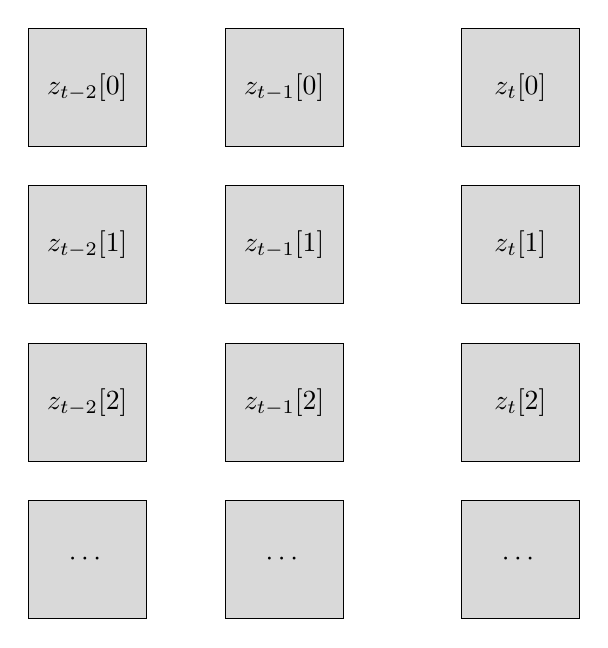
\begin{tikzpicture}[every text node part/.style={align=center}]
    % Preliminaries
    \usetikzlibrary{shapes.geometric, arrows, shapes.multipart}
    \tikzstyle{box} = [rectangle, minimum width=1.5cm, minimum height=1.5cm, text centered, draw=black, fill=gray!30]
    %\tikzstyle{box} = [rectangle, minimum width=1.5cm, minimum height=1cm, text centered, draw=black, fill=orange!30]
    \tikzstyle{strat} = [rectangle, minimum width=1.5cm, minimum height=1cm, text centered, draw=white, fill=white]
    \tikzstyle{arrow} = [thick,->,>=stealth]
    % Field Processing Flow
    %\node (field_strat) [strat] {Field \\ Processing};
    \node (z_tm2_0) [box] {$z_{t-2}[0]$};
    \pause
    \node (z_tm2_1) [box,below of=z_tm2_0,yshift=-1cm] {$z_{t-2}[1]$};
    \pause
    \node (z_tm2_2) [box,below of=z_tm2_1,yshift=-1cm] {$z_{t-2}[2]$};
    \pause
    \node (z_tm2_3) [box,below of=z_tm2_2,yshift=-1cm] {$\cdots$};
    \pause
    \node (z_tm1_0) [box,right of=z_tm2_0,xshift=1.5cm] {$z_{t-1}[0]$};
    \node (z_tm1_1) [box,below of=z_tm1_0,yshift=-1cm] {$z_{t-1}[1]$};
    \node (z_tm1_2) [box,below of=z_tm1_1,yshift=-1cm] {$z_{t-1}[2]$};
    \node (z_tm1_3) [box,below of=z_tm1_2,yshift=-1cm] {$\cdots$};
    \pause
    \node (z_t_0) [box,right of=z_tm1_0,xshift=2cm] {$z_t[0]$};
    \node (z_t_1) [box,below of=z_t_0,yshift=-1cm] {$z_t[1]$};
    \node (z_t_2) [box,below of=z_t_1,yshift=-1cm] {$z_t[2]$};
    \node (z_t_3) [box,below of=z_t_2,yshift=-1cm] {$\cdots$};
    \pause
  \end{tikzpicture}
\end{frame}

\begin{frame}{Leslie to Euler-Lotka}
  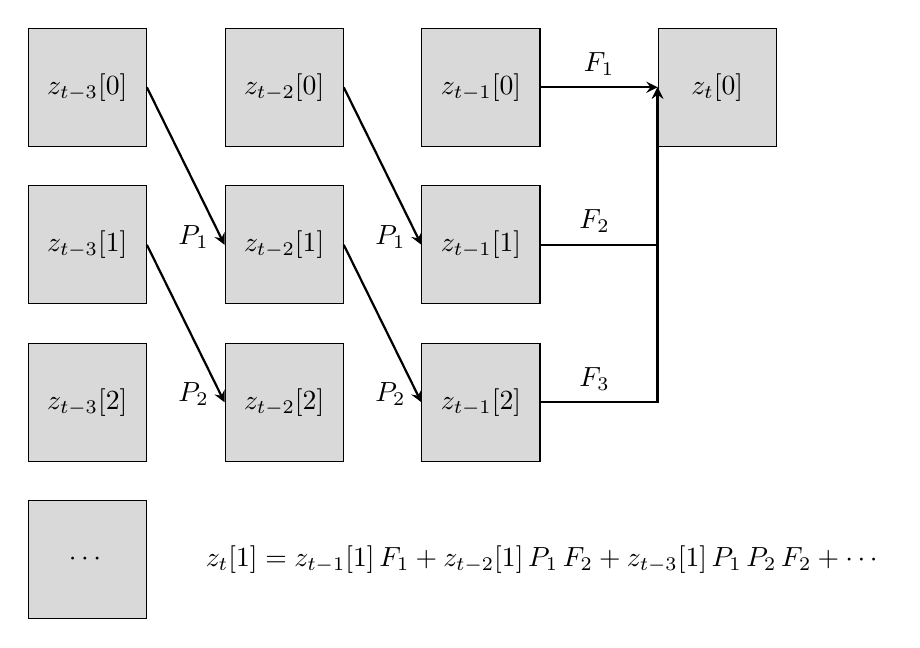
\begin{tikzpicture}[every text node part/.style={align=center}]
    % Preliminaries
    \usetikzlibrary{shapes.geometric, arrows, shapes.multipart}
    \tikzstyle{box} = [rectangle, minimum width=1.5cm, minimum height=1.5cm, text centered, draw=black, fill=gray!30]
    %\tikzstyle{box} = [rectangle, minimum width=1.5cm, minimum height=1cm, text centered, draw=black, fill=orange!30]
    \tikzstyle{mathbox} = [rectangle, minimum width=1.5cm, minimum height=1cm, text centered, draw=white, fill=white]
    \tikzstyle{arrow} = [thick,->,>=stealth]
    % Field Processing Flow
    %\node (field_strat) [strat] {Field \\ Processing};
    \node (z_tm3_0) [box] {$z_{t-3}[0]$};
    \node (z_tm3_1) [box,below of=z_tm3_0,yshift=-1cm] {$z_{t-3}[1]$};
    \node (z_tm3_2) [box,below of=z_tm3_1,yshift=-1cm] {$z_{t-3}[2]$};
    \node (z_tm3_3) [box,below of=z_tm3_2,yshift=-1cm] {$\cdots$};
    
    \node (z_tm2_0) [box,right of=z_tm3_0,xshift=1.5cm] {$z_{t-2}[0]$};
    \node (z_tm2_1) [box,below of=z_tm2_0,yshift=-1cm] {$z_{t-2}[1]$};
    \node (z_tm2_2) [box,below of=z_tm2_1,yshift=-1cm] {$z_{t-2}[2]$};
    %\node (z_tm2_4) [box,below of=z_tm2_3,yshift=-1cm] {$\cdots$};
    
    \node (z_tm1_0) [box,right of=z_tm2_0,xshift=1.5cm] {$z_{t-1}[0]$};
    \node (z_tm1_1) [box,below of=z_tm1_0,yshift=-1cm] {$z_{t-1}[1]$};
    \node (z_tm1_2) [box,below of=z_tm1_1,yshift=-1cm] {$z_{t-1}[2]$};
    %\node (z_tm1_4) [box,below of=z_tm1_3,yshift=-1cm] {$\cdots$};
    
    \node (z_t_0) [box,right of=z_tm1_0,xshift=2cm] {$z_t[0]$};
    
    \draw [arrow] (z_tm3_0.east) to node[xshift=.1cm,yshift=-.9cm] {$P_1$} (z_tm2_1.west);
    \pause
    \draw [arrow] (z_tm3_1.east) to node[xshift=.1cm,yshift=-.9cm] {$P_2$} (z_tm2_2.west);
    %\draw [arrow] (z_tm2_3.east) to (z_tm1_4.west);
    \pause

    \draw [arrow] (z_tm2_0.east) to node[xshift=.1cm,yshift=-.9cm] {$P_1$} (z_tm1_1.west);
    \draw [arrow] (z_tm2_1.east) to node[xshift=.1cm,yshift=-.9cm] {$P_2$} (z_tm1_2.west);
    %\draw [arrow] (z_tm1_3.east) to (z_t_4.west);
    \pause
    
    \draw [arrow] (z_tm1_0.east) to node[yshift=.3cm] {$F_1$} (z_t_0.west);
    \draw [arrow] (z_tm1_1.east) -| node[yshift=.3cm,xshift=-.8cm] {$F_2$} (z_t_0.west);
    \draw [arrow] (z_tm1_2.east) -| node[yshift=.3cm,xshift=-.8cm] {$F_3$} (z_t_0.west);
    
    \node (euler_lotka) [mathbox,right of=z_tm3_3,xshift=4.8cm] {$z_t[1] = z_{t-1}[1] \, F_1 + z_{t-2}[1] \, P_1 \, F_2 + z_{t-3}[1] \, P_1 \, P_2 \, F_2 + \cdots$};
    
  \end{tikzpicture}
\end{frame}

\begin{frame}{Leslie to Euler-Lotka}
  $y_t \equiv z_t[1]$\\
  \vspace{.5cm}
  $y_t = y_{t-1} \, F_1 + y_{t-2} \, S_1 \ F_2 + y_{t-2} \, P_1 \, P_2 \, F_3 + \cdots = \displaystyle\sum\limits_{j=1}^{J} y_{t-j-1} \, l_j \, F_j$\\
  \vspace{.5cm}
  Posit an exponential solution\\
  \vspace{.5cm}
  $y_{t-j-1} = \frac{y_t}{\lambda^{j+1}}$\\
  \vspace{.5cm}
  $1 = \displaystyle\sum\limits_{j=1}^{J} \frac{l_j \, F_j}{\lambda^{j+1}}$\\
  %$l_j = \displaystyle\prod\limits_{i=1}^{j-1} P_k$
\end{frame}

\begin{frame}{Backup: derivatives of matrices}
  The right eigenvectors of $\mathbf{A}$ are defined by the equation\\
  \vspace{.5cm}
  $\mathbf{A} \, \mathbf{w}^{(m)} = \lambda^{(m)} \, \mathbf{w}^{(m)}$\\
  \vspace{.5cm}
  The left eigenvectors of $\mathbf{A}$ are defined by the equation\\
  ${\mathbf{v}^{(m)}}^{\dagger} \, \mathbf{A} =	{\mathbf{v}^{(m)}}^{\dagger} \, \lambda^{(m)}$\\
  \vspace{.5cm}
  Taking an exterior derivative of the top equation yields\\
  \vspace{.5cm}
  $\mathrm{d}\mathbf{A} \, \mathbf{w}^{(m)} + \mathbf{A} \, \mathrm{d}\mathbf{w}^{(m)}= \mathrm{d}\lambda^{(m)} \, \mathbf{w}^{(m)} + \lambda^{(m)} \, \mathrm{d}\mathbf{w}^{(m)}$\\
\end{frame}

\begin{frame}{Backup: derivatives of matrices}
  Now take the inner product with respect to $\greekbf{v}^{(n)}$ (i.e., pre-multiply by ${\greekbf{v}^{(n)}}^{\dagger}$ and rearrange terms)\\
  \vspace{.5cm}
  ${\mathbf{v}^{(n)}}^{\dagger} \, \mathrm{d}\mathbf{A} \, \mathbf{w}^{(m)} = {\mathbf{v}^{(n)}}^{\dagger} \, \mathrm{d}\lambda^{(m)} \, \mathbf{w}^{(m)} + {\mathbf{v}^{(n)}}^{\dagger} \left(\lambda^{(m)} - \mathbf{A} \right) \mathrm{d}\mathbf{w}^{(m)}$\\
  \vspace{.5cm}
  If $m=n$ the last term on the right vanishes\\
  \vspace{.5cm}
  ${\mathbf{v}^{(m)}}^{\dagger} \, \mathrm{d}\mathbf{A} \, \mathbf{w}^{(m)} = {\mathbf{v}^{(m)}}^{\dagger} \, \mathrm{d}\lambda^{(m)} \, \mathbf{w}^{(m)}$\\
\end{frame}

\begin{frame}{Backup: derivatives of matrices}
  Solving for $\mathrm{d}\lambda^{(m)}$ yields\\
  \vspace{.5cm}
  $\mathrm{d}\lambda^{(m)} = \frac{{\mathbf{v}^{(m)}}^{\dagger} \, \mathrm{d}\mathbf{A} \, \mathbf{w}^{(m)}}{\psi^{(m)}}$\\
  \vspace{.5cm}
  where $\psi^{(m)}=\mathbf{v}^{(m)\dagger} \, \mathbf{w}^{(m)}$ is the inner product of the left and right eigenvectors of $\lambda^{(m)}$.\\
  \vspace{.5cm}
  Representing this in terms of the matrix element $A_{ij}$ yields\\
  \vspace{.5cm}
  $\frac{\partial \lambda^{(m)}}{\partial A_{ij}} = \frac{v^{(m)}_i \, w^{(m)}_j}{\psi^{(m)}}$
\end{frame}

\end{document}
